\documentclass{beamer}

\mode<presentation>
\usetheme{Madrid}

\usepackage[spanish]{babel}
\usepackage[utf8]{inputenc}
\usepackage[T1]{fontenc} % hyphenation 
\usepackage{times}
\usepackage{tikz}
\usepackage{booktabs}

\setbeamercovered{dynamic}

\title[GIS]{Introducción a Sistemas de Información Geográfica}
\subtitle[]{Curso de Zonificación Vitícola y Viticultura de Precisión}


\author[G.F. Olmedo]{Guillermo Federico Olmedo}

\institute[INTA] % (optional, but mostly needed)
{ Laboratorio de Geomática\\
  Recursos Naturales\\
  INTA EEA Mendoza\\
  \vskip10pt
\begin{columns}
	\column{.5\textwidth}
	\begin{flushright}
		
\includegraphics[width=1.7cm]{IMGs/logoINTA}
	\end{flushright}
	\column{.5\textwidth}
	\begin{flushleft}
		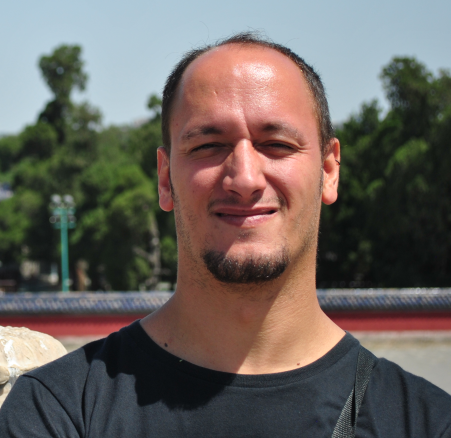
\includegraphics[width=1.7cm]{IMGs/yo}
	\end{flushleft}
\end{columns}  
}

\date[FCA, 16-20/05/2016]{Fac. de Cs. Agrarias, 16 al 20 de mayo de 2016}

\pgfdeclareimage[height=0.5cm]{university-logo}{IMGs/logoINTA}
\logo{\pgfuseimage{university-logo}}

%\beamerdefaultoverlayspecification{<+->}


\begin{document}

\begin{frame}[plain]
  \titlepage
\end{frame}

\begin{frame}{Outline}
	\tableofcontents[pausesections]
	% You might wish to add the option [pausesections]
\end{frame}

\section{Introducción}

\begin{frame}{Que es un SIG?}
Un Sistema de Información Geográfica (SIG o GIS)\footnote{{\footnotesize }Fuente: Wikipedia}, es una integración organizada de \textit{hardware}, \textit{software} y datos \textit{geográficos} diseñada para capturar, almacenar, manipular y analizar información \textit{geográficamente referenciada} con el fin de resolver problemas complejos de planificación y gestión.
\end{frame}

\begin{frame}[plain]{}
	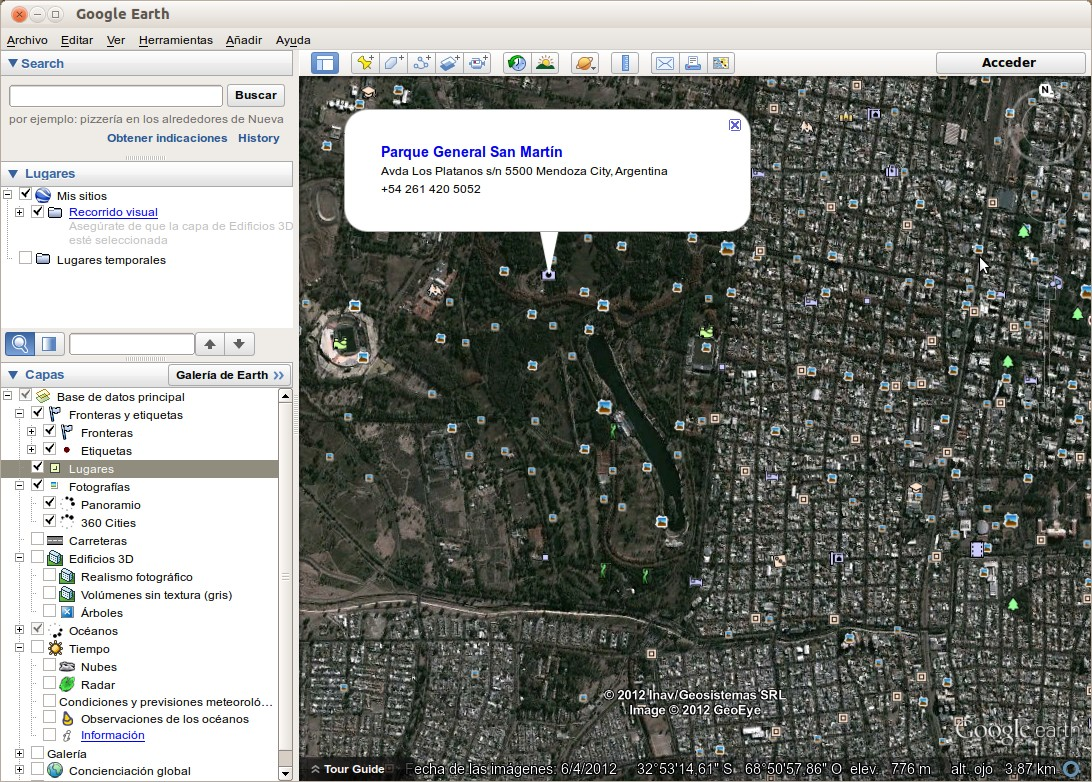
\includegraphics[width=\textwidth]{IMGs/googleea}
\end{frame}

\begin{frame}[plain]{}
	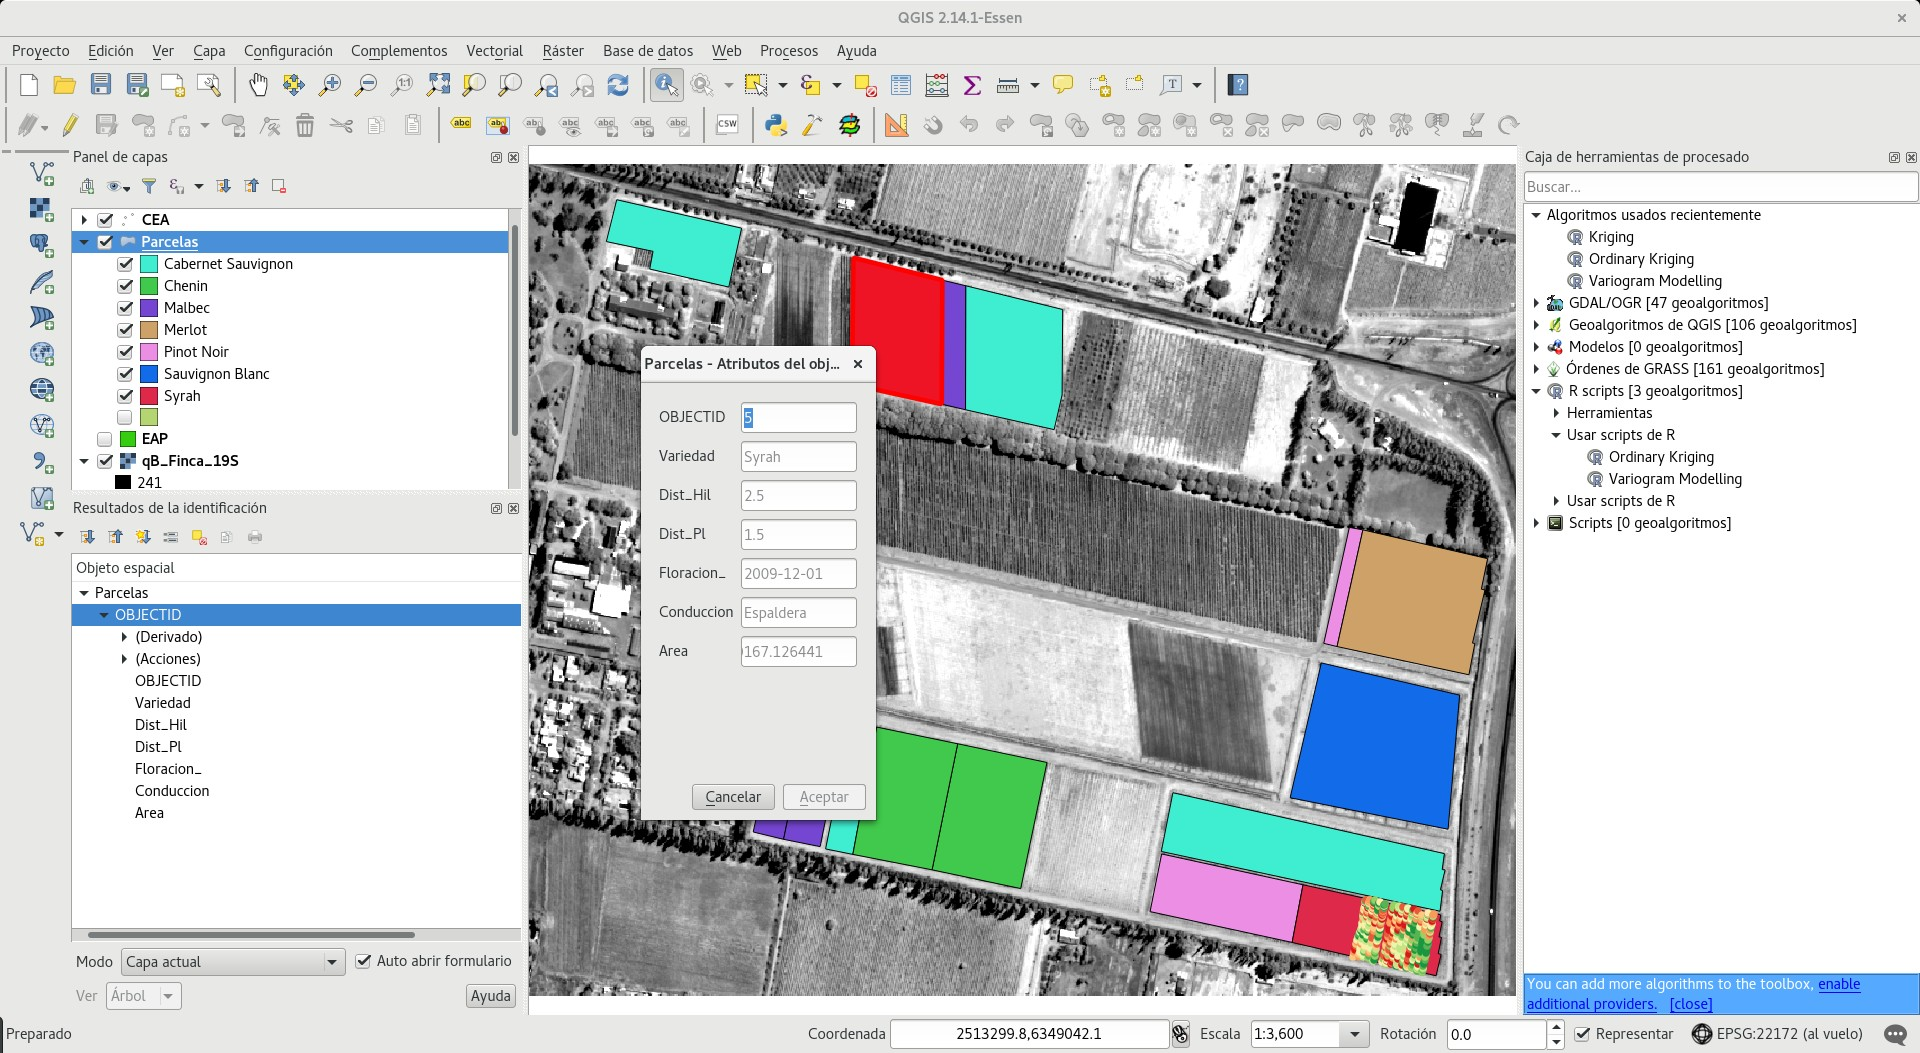
\includegraphics[width=\textwidth]{IMGs/QGIS}
\end{frame}

\begin{frame}[plain]{}
	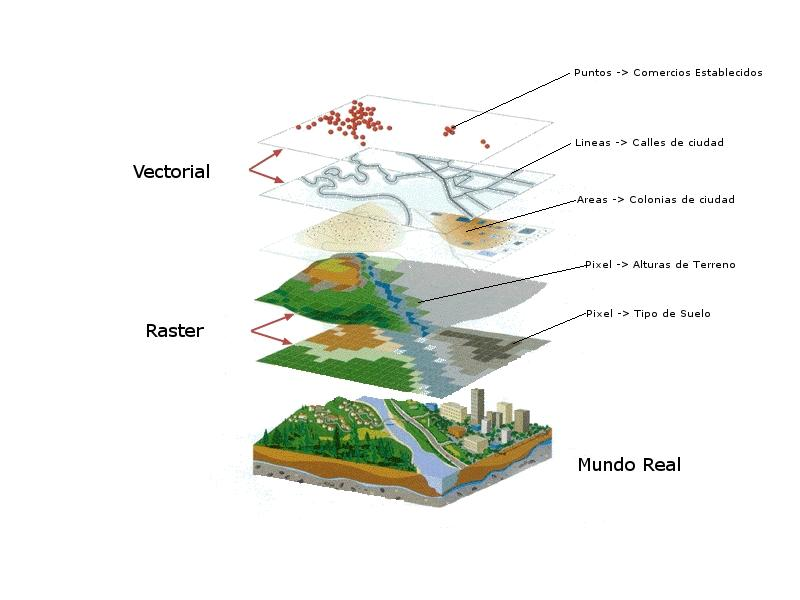
\includegraphics[width=\textwidth]{IMGs/GIS}
\end{frame}

\section{Información}

\begin{frame}{Tipos de información espacial}{Raster}
	\begin{columns}
		\column{.45\textwidth}
			\begin{itemize}
				\item Es una matriz ordenada de celdas en filas y columnas. Cada celda (píxel) toma un valor único. Generalmente representan datos continuos, son más importantes las propiedades del espacio que la precisión de la localización.
				\item<6> En algunos formatos se suelen “apilar” diferentes variables, pudiendo luego ver el valor de las variables para una misma ubicación.
			\end{itemize}
		\column{.45\textwidth}
		    \begin{figure}
		    	\includegraphics<1>[width=0.8\textwidth]{IMGs/raster1}
		    	\includegraphics<2>[width=0.8\textwidth]{IMGs/raster2}
		    	\includegraphics<3>[width=0.8\textwidth]{IMGs/raster3}
		    	\includegraphics<4>[width=0.8\textwidth]{IMGs/raster4}
		    	\includegraphics<5>[width=0.8\textwidth]{IMGs/raster5}
		    	\includegraphics<6>[width=0.9\textwidth]{IMGs/multi}
		    \end{figure} 
	\end{columns}
\end{frame}

\begin{frame}{Tipos de información espacial}{Tipos de Raster}
	\begin{itemize}[<+->]
		\item Raster continuos\\
		Generalmente representan una propiedad física continua. 
		Por ejemplo: la altitud, la reflectancia a una longitud de onda determinada o el valor de NDVI.
		\item Raster temáticos\\
		Los píxels toman un valor discreto que corresponde a una clase. Una variación de estos son los raster booleanos, que toman valor 1 o 0 de acuerdo a la pertenencia o no a una clase.
		Por ej.: zonas de alto o bajo vigor; suelos con freática o no.
	\end{itemize}
\end{frame}

\begin{frame}{Tipos de información espacial}{Vectorial}
	\begin{columns}
		\column{.45\textwidth}
		\begin{itemize}[<+->]
			\item Pueden ser puntos, líneas o polígonos. 
			\item Generalmente representan datos discretos, donde la precisión de la localización en el factor más importante. 
			\item Cada entidad esta ligada a una base de datos.
		\end{itemize}
		\column{.45\textwidth}
		\begin{figure}
			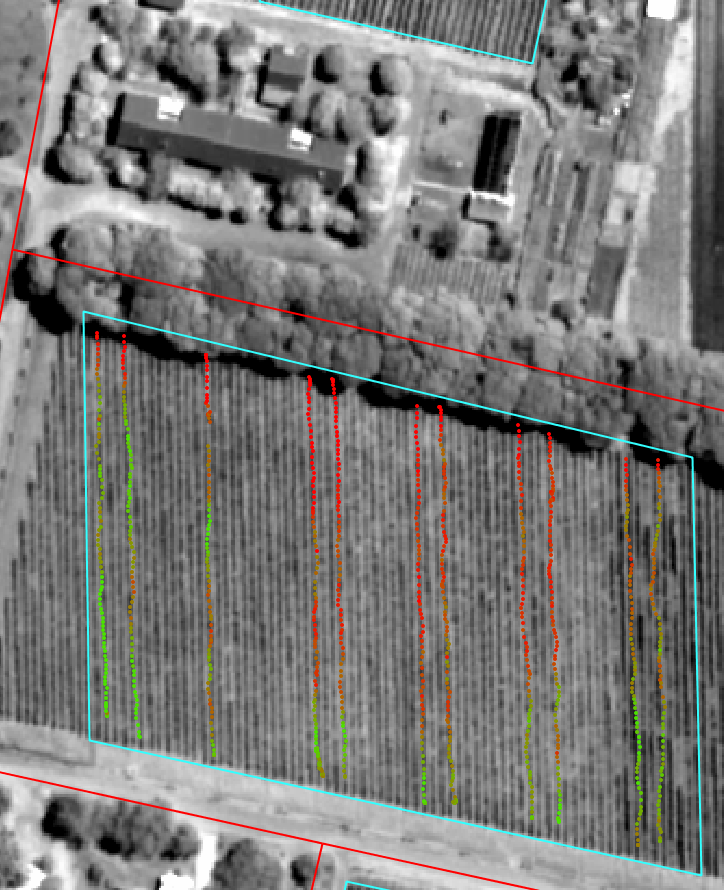
\includegraphics[width=0.8\textwidth]{IMGs/vector}
		\end{figure}
	\end{columns}
\end{frame}

\begin{frame}{Tipos de información espacial}
	\begin{columns}[t]
		\column{.45\textwidth}
		Raster
		\begin{itemize}[<+->]
			\item Información continua
			\item Análisis entre capas
		\end{itemize}
		\column{.45\textwidth}
		Vectorial
		\begin{itemize}[<+->]
			\item Información discreta
			\item Menos volumen de datos
			\item Representación independiente de la escala
		\end{itemize}
	\end{columns}
\end{frame}

\section{Sistemas de Referencia}

\begin{frame}{Sistemas de Referencia}
	\begin{itemize}[<+->]
		\item Es un conjunto de normas y convenciones que permite ubicar un punto en el espacio.
		\item Está compuesto por: 
		\begin{itemize}
			\item Geoide de Referencia
			\item Sistema de Coordenadas
			\item Proyección Cartográfica
			\item Marco de Referencia - Datum 
		\end{itemize}
	\end{itemize}
\end{frame}

\begin{frame}{Sistemas de Referencia}{Geoide de Referencia}
	\begin{columns}[]
		\column{.45\textwidth}
		\begin{itemize}
			\item Internacional de 1924
			\item WGS 1984
		\end{itemize}
		\column{.45\textwidth}
		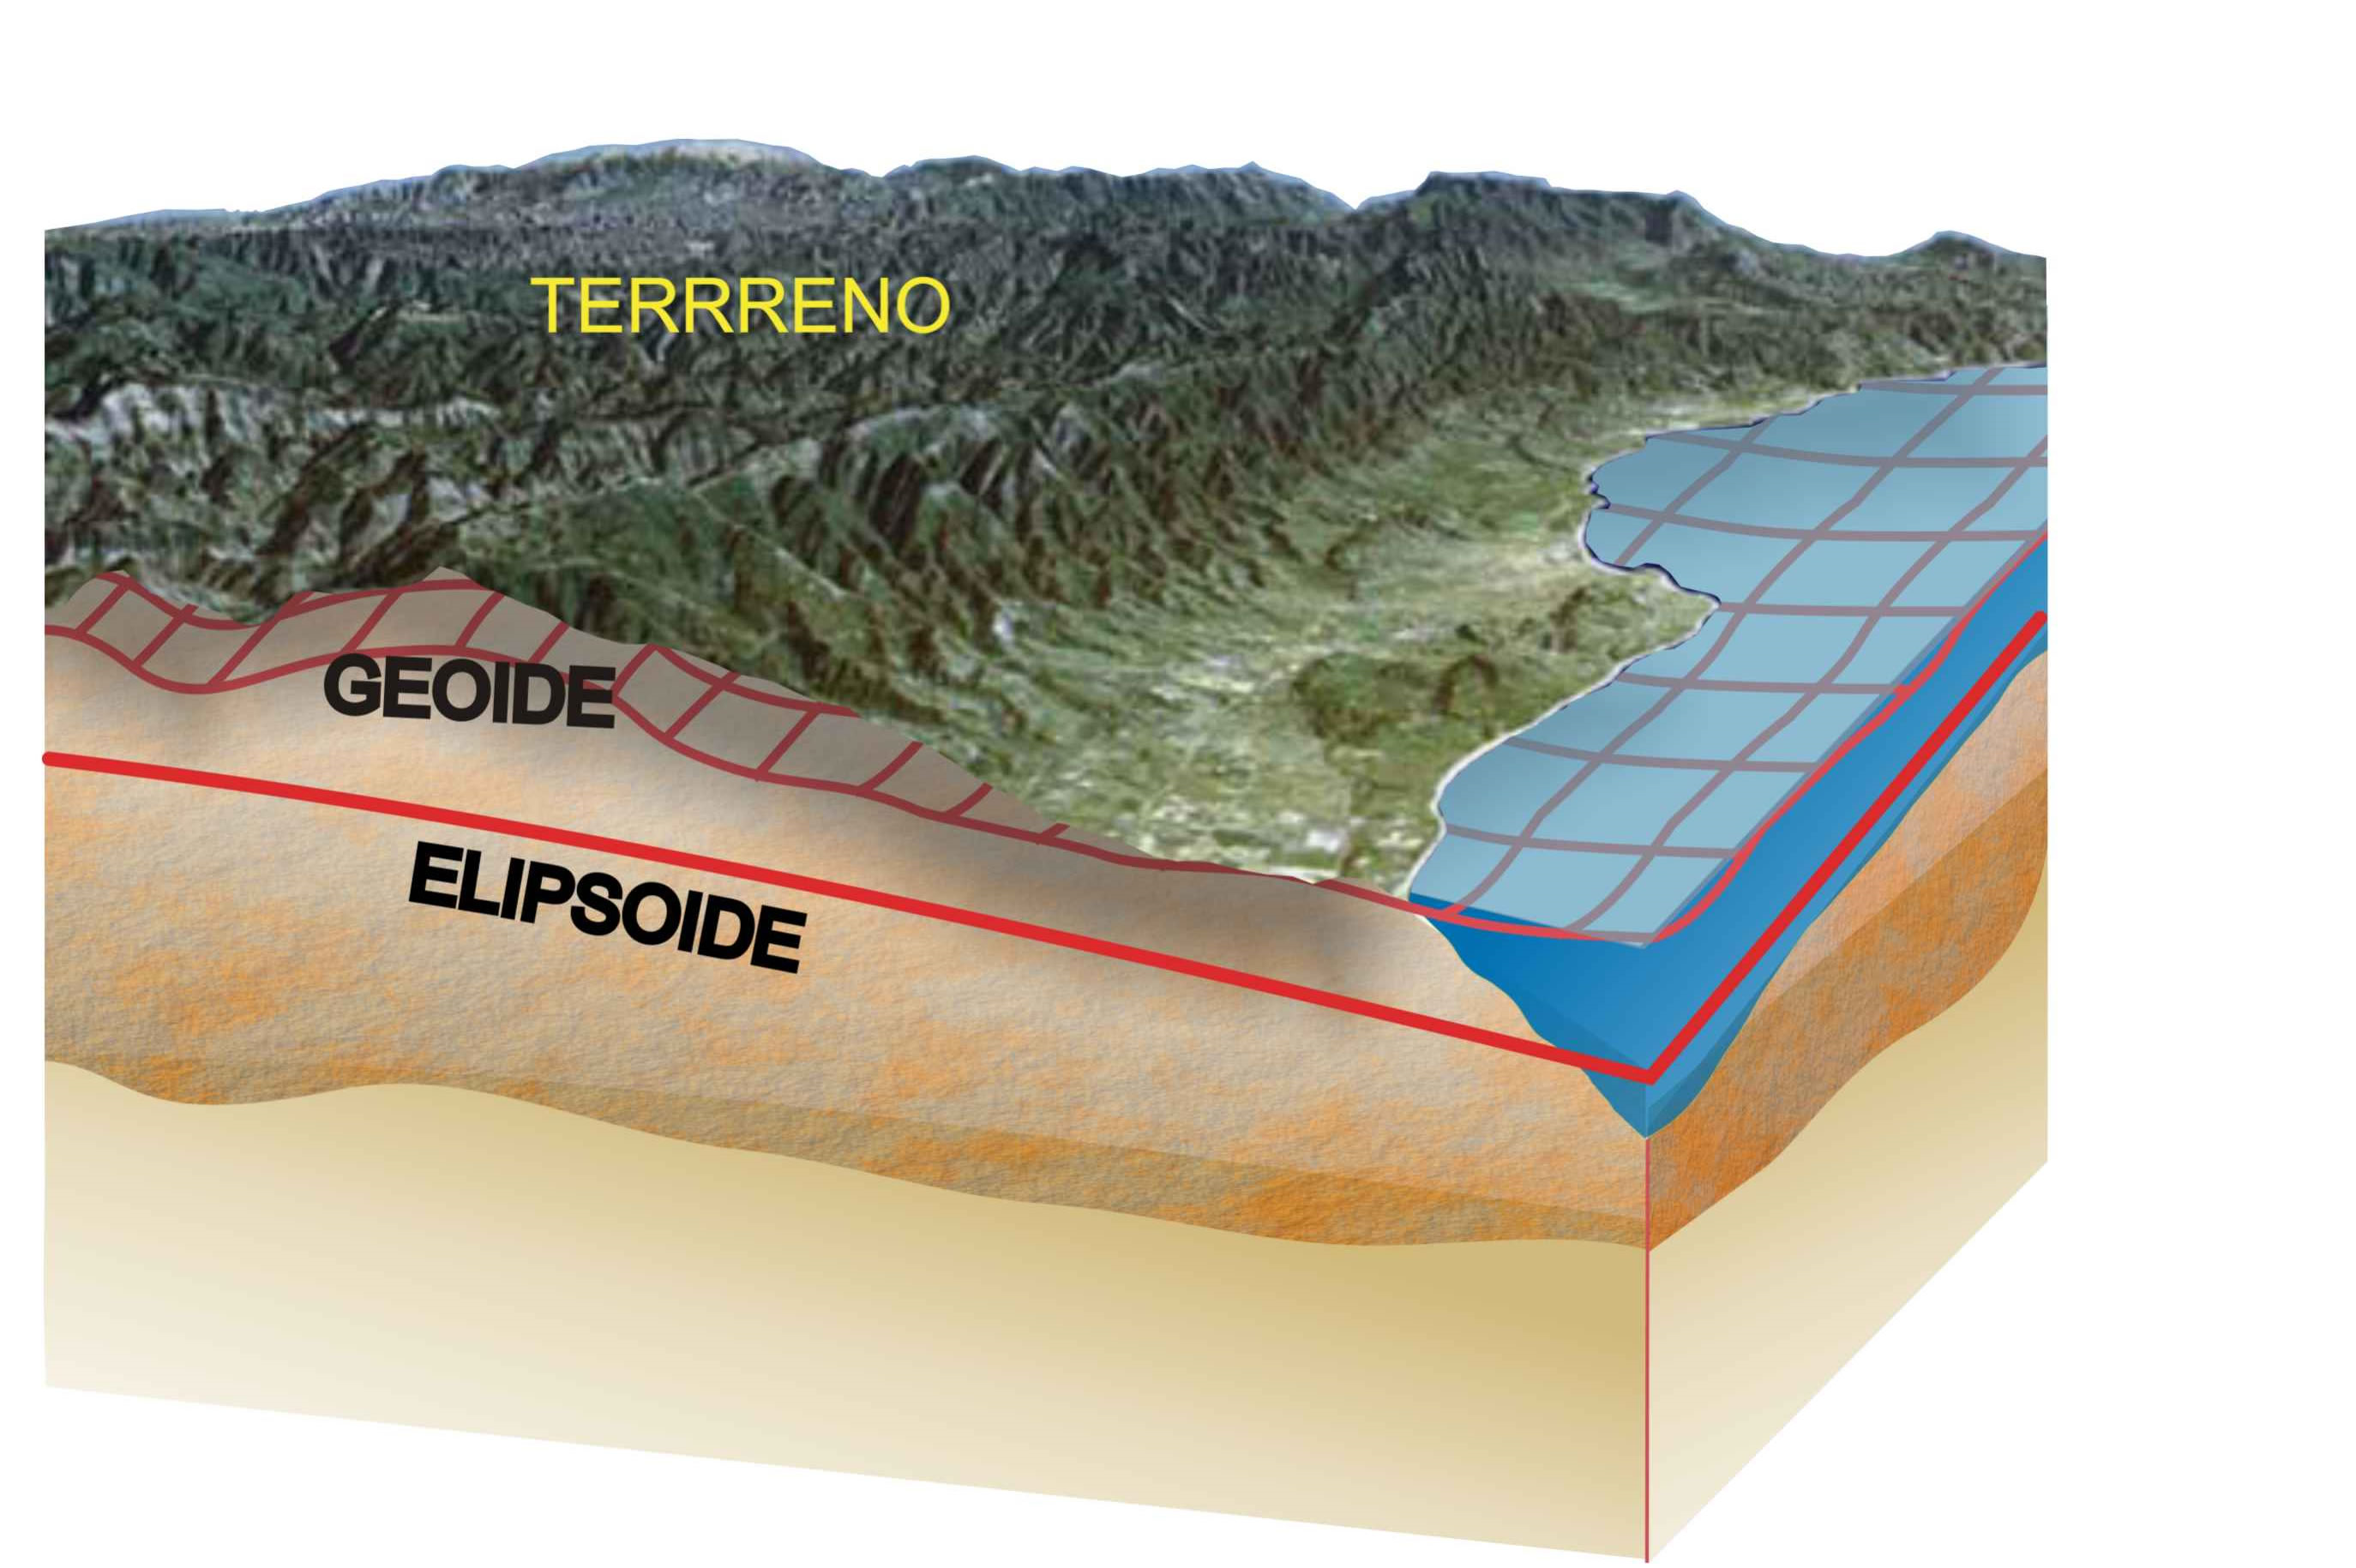
\includegraphics[width=\textwidth]{IMGs/geoide}
	\end{columns}
\end{frame}

\begin{frame}{Sistemas de Referencia}{Sistema de Coordenadas}
		\begin{columns}[]
			\column{.45\textwidth}
			Coordenadas Geográficas
			\begin{itemize}
				\item La latitud mide el ángulo entre cualquier punto y el ecuador.
				\item La longitud mide el ángulo a lo largo del ecuador desde cualquier punto de la Tierra.
			\end{itemize}
		\column{.45\textwidth}
		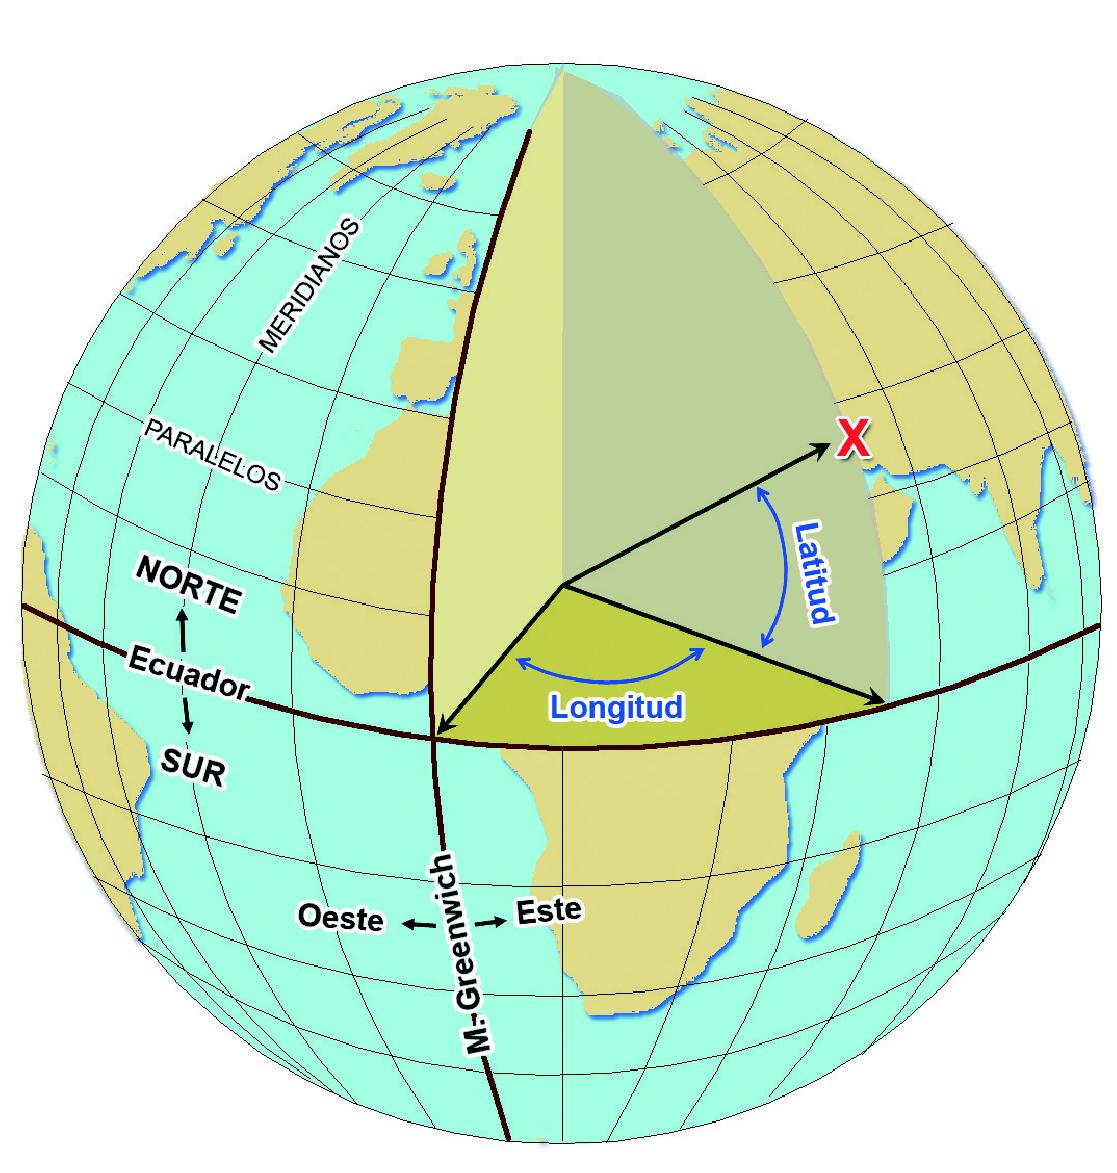
\includegraphics[width=\textwidth]{IMGs/latlon}
	\end{columns}
\end{frame}

\begin{frame}{Sistemas de Referencia}{Proyección cartográfica}
		\begin{itemize}[<+->]
			\item Proyecciones conformes: conservan los ángulos. Se utilizan para la navegación. Son útiles para las representaciones de las características geológicas.
			\item Proyecciones equivalentes: conservan las superficies.
			\item Proyecciones equidistantes: conservan las distancias.
		\end{itemize}	
			Según el tipo:
		\begin{itemize}
			\item Proyecciones azimutales o cenitales.
			\item Proyecciones cilíndricas.
			\item Proyecciones cónicas. 
		\end{itemize}
\end{frame}

\begin{frame}{Sistemas de Referencia}{Coordenadas Planas}
		\begin{itemize}
			\item Coordenadas UTM
		\end{itemize}
\end{frame}

\begin{frame}{Sistemas de Referencia}{Marco de referencia - Datum}
		Es un conjunto de puntos sobre la superficie terrestre que materializa el sistema de referencia.
		\begin{itemize}
			\item Chos Malal 1914
			\item Campo Inchauspe 1969
			\item PosGAR 1994
			\item PosGAR 1998
		\end{itemize}
\end{frame}

\begin{frame}{Sistemas de Referencia}{Marco Oficial Argentino}
			\begin{itemize}
				\item  POSGAR98 Faja 2
			\end{itemize}
\end{frame}

\begin{frame}{Sistemas de Referencia}{Clasificaciones de SRCs}
	European Petroleum Survey Group (EPSG) \footnote{desde 2005: OGP}\\
	
	Grupo científico vinculado a la industria petrolera europea que compiló los parámetros de diferentes sistemas de coordenadas, proyecciones, y datums.	El resultado fue el Sistema de Identificador de Referencia Espacial (SRID). Este puede consultarse en \url{http://spatialreference.org} 
	\begin{table}
	\centering
		\begin{tabular}{l|c}
		\toprule
		Sistema           & EPSG  \\
		\midrule
		geográficas WGS84 & 4326  \\
		UTM 19 S          & 32719 \\
		POSGAR94 Faja 2   & 22172 \\
		POSGAR98 Faja 2   & 22182 \\
		Campo Ichauspe 2  & 22192 \\
		Google Mercator   & 3857 
		\bottomrule
		\end{tabular}
	\end{table}	
\end{frame}

\section{Formatos}

\begin{frame}{Los formatos}
	\begin{columns}[t]
			\column{.45\textwidth}
			Formatos Vectoriales
			\begin{itemize}
				\item Shapefile 
				\item KML / KMZ 
				\item DXF
				\item GDBs (Features)
			\end{itemize}
			\column{.45\textwidth}
			Formatos Raster
			\begin{itemize}
				\item IMG (Erdas Imagine)
				\item TIF / GeoTIFF
				\item FastFormat
				\item GRID
				\item GDBs (BLOBs)
			\end{itemize}
	\end{columns}
\end{frame}

\begin{frame}{Formatos Vectoriales}
	\begin{itemize}[<+->]
		\item Shapefile: Formato más difundido. Estándar de facto. Es un formato propietario abierto desarrollado por ESRI. Almacena los datos geográficos y los atributos asociados a ellos. Consta de varios archivos:
		\begin{itemize}
			\item .shx: índice
			\item .dbf: datos temáticos
			\item .prj: proyección cartográfica
			\item .shp.xml: metadatos
			\item y otros \ldots
		\end{itemize}.shp: entidades geográficas
		\item Problemas: No almacena topología. Suele quedarse alguno al enviar por correo.
	\end{itemize}
\end{frame}

\begin{frame}{Formatos Vectoriales}
	\begin{itemize}[<+->]
		\item Kml / Kmz: Utilizado por Google Earth, almacena datos en 3 dimensiones. Almacena poca información temática. Basado en xml. Estándar abierto (OGC). Da algunos problemas al convertir a otros formatos.
		\item DXF: Formato CAD. No almacena proyecciones cartográficas.
		\item Geodatabases: Es la tendencia actual. Almacenan topologías y pueden compartir información. Las relaciones entre las capas también son almacenadas.
	\end{itemize}
\end{frame}

\begin{frame}{Formatos raster}
	\begin{itemize}[<+->]
		\item IMG: Desarrollado por Leica. Formato abierto, bastante generalizado. Admite compresión.
		\item TIFF / GeoTIFF: Desarrollado por el JPL-NASA. No admite compresión. Formato abierto y muy generalizado. Es un TIFF con información geográfica, puede ser abierto como un TIFF normal. 
		\item FastFormat: Formato de distribución de imágenes Landsat. Casi en desuso. Incluye el header de la imagen.
		\item GRID: Desarrollado por ESRI. Problemas de interconvertibilidad. Suele corromperse al copiarlo a otra carpeta.
		\item GDB: Los raster presentan problemas al almacenarlos en una GDB por las limitaciones de volumen de datos de las mismas.
	\end{itemize}
\end{frame}

\begin{frame}{Formatos Web}
	\begin{itemize}[<+->]
		\item WMS (Web Map Service) permite incorporar a través de internet, información geográfica a un GIS. 
		\item WMS no “sirve” directamente los datos espaciales, sino que envía pequeños mosaicos como imagen de la información.
		\item De esta forma la información es protegida y sólo se puede incorporar para visualización. Por lo que no es posible ni analizarla ni editarla.
		\item Existe una versión del protocolo que permite la edición, llamado WFS.  
	\end{itemize}
\end{frame}

\begin{frame}{Formatos Web}
	\begin{itemize}[<+->]
		\item El INTA pone a disposición de los usuarios en formato WMS mucha información como mapas de suelos, cobertura vegetal, información climática a través de la plataforma geoINTA.
		\item \url{http://geointa.inta.gov.ar/geoserver/wms}
		\item Esta información también puede visualizarse en el navegador web en geointa.inta.gob.ar
	\end{itemize}
\end{frame}

\end{document}

